%!TEX root = ../dissertation.tex

\chapter{Results and Discussion}
\label{cha4:results}
\section{Simulator}
As it was specified on Figure \ref{cha1:sec1:fig:curr_eye_model}, the current eye prototype contains a baseline length of $53.7 \ mm$ on the torsional axis. To make the comparisons easier, this baseline was also used in the simulator.
\subsection{Rotation estimation error}
On experiment 1, the variance used on the Gaussian distribution was $4 \degree$ so to simulate the saccade amplitudes of the human eye. On experiment 2, the variance was $15 \degree$, in order to understand how the estimation algorithm works in wider amplitude ranges.
\subsubsection{Simulation Parameters}
The following parameters were used to run the simulation. Zmax and Zmin refer to the range in which points are simulated explained on section \ref{rienreive}.
\begin{itemize}
	\item Maximum Matches : $30$
	\item False Matches : $10 \%$ of maximum matches
	\item Good Matches : $50 \%$ of the maximum matches
	\item Gaussian Noise $\sigma^2$ : $10 \ px$
	\item Number of saccades: $45$
	\item Zmin : $0.05 m$
	\item Zmax : $5 m$
\end{itemize}
\subsubsection{Experiment 1 - Saccade amplitudes generated with $\sigma^2 = 4 \degree $}
Figures \ref{cha5:sec1:10anglex}, \ref{cha5:sec1:10angley} and \ref{cha5:sec1:10anglez}, show the error, computed as \ref{firenr}, from the estimation of the rotation per saccade amplitudes on the horizontal, vertical and torsional axis, respectively. The amplitudes were generated randomly around a specific axis in a normal distribution with variance $\sigma^2 = 4 \degree$. Table \ref{cha5:sec1:10angleaxist}, shows the corresponding mean error in degrees per axis for each of the methods.

\begin{minipage}{0.33\textwidth}
	\centering
	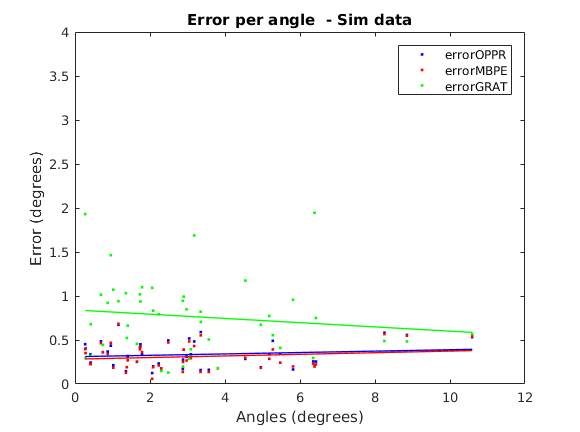
\includegraphics[width=\textwidth]{images/sim/10anglex.png}
	\captionof{figure}{Error per saccade amplitude (in degrees) under simulation on the horizontal axis.}
	\label{cha5:sec1:10anglex}
\end{minipage}
\begin{minipage}{0.33\textwidth}
	\centering
	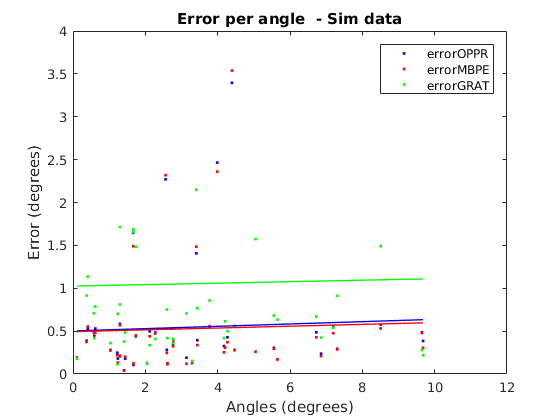
\includegraphics[width=\textwidth]{images/sim/10angley.png}
	\captionof{figure}{Error per saccade amplitude (in degrees) under simulation on the vertical axis.}
	\label{cha5:sec1:10angley}
\end{minipage}
\begin{minipage}{0.33\textwidth}
	\centering
	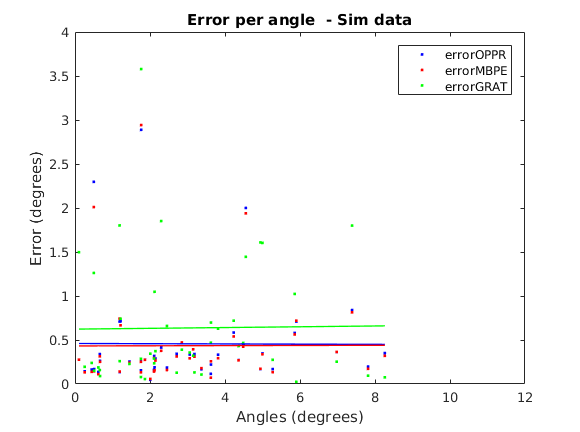
\includegraphics[width=\textwidth]{images/sim/10anglez.png}
	\captionof{figure}{Error per saccade amplitude (in degrees) under simulation on the torsional axis.}
	\label{cha5:sec1:10anglez}
\end{minipage}
\begin{table}
	\centering
	\begin{tabular}{| l | l | l | l |}
		\hline
		Method & X Mean & Y Mean & Z Mean \\
		\hline
		OPPR &  0.33 \degree & 0.54 \degree & 0.46 \degree \\
		\hline
		MBPE &  0.31 \degree & 0.52 \degree & 0.44 \degree\\
		\hline
		GRAT &  0.77 \degree & 1.05 \degree & 0.64 \degree\\ 
		\hline
	\end{tabular}
	\captionof{table}{Mean error (in degrees) per method and per axis.}
	\label{cha5:sec1:10angleaxist}
\end{table}		

Figure \ref{cha5:sec1:10angle} shows the error from the estimation of the rotation per saccade amplitudes randomly executed around all axis simultaneously. Table \ref{cha5:sec1:10anglet} shows the mean error and standard deviation for this experiment for each of the methods.

\begin{minipage}{0.5\textwidth}
	\centering
	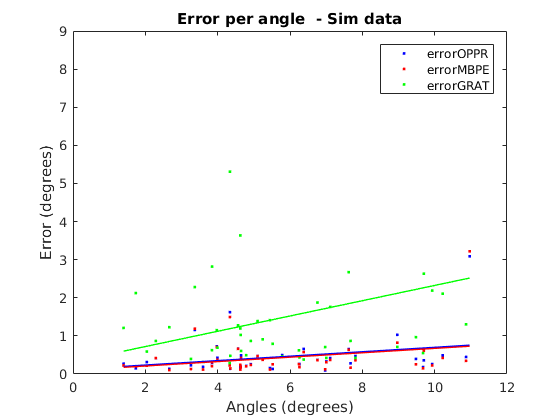
\includegraphics[width=\textwidth]{images/sim/10angle.png}
	\captionof{figure}{Error per saccade amplitude (in degrees) under simulation.}
	\label{cha5:sec1:10angle}
\end{minipage}
\begin{minipage}{0.5\textwidth}
	\centering
	\begin{tabular}{| l | l | l |}
			\hline
			Method & Mean & Standard Deviation \\
			\hline
			OPPR &  0.45 \degree & 0.49 \degree \\
			\hline
			MBPE &  0.42 \degree & 0.50 \degree \\
			\hline
			GRAT &  1.47 \degree & 1.76 \degree \\ 
			\hline
	\end{tabular}
	\captionof{table}{Mean error and standard deviation (in degrees) of the experiment on the left per each method tested}
	\label{cha5:sec1:10anglet}
\end{minipage}\\

Robust estimation was applied to filter out wrong matches and detected a $15.55 \%$ of them from the whole set of matches.

\subsubsection{Experiment 2 - Saccade amplitudes generated with $\sigma^2 = 15 \degree $}

Just like Experiment 1, Figure \ref{cha5:sec1:45angle} shows the error per  amplitude in degrees from random saccades around around all axis simultaneously, generated in a normal distribution with variance $\sigma^2 = 15 \degree $. Table \ref{cha5:sec1:45anglet} presents the respective mean error and standard deviation. Robust estimation detected a $ 22.55 \%$ of bad matches.

\begin{minipage}{0.5\textwidth}
	\centering
	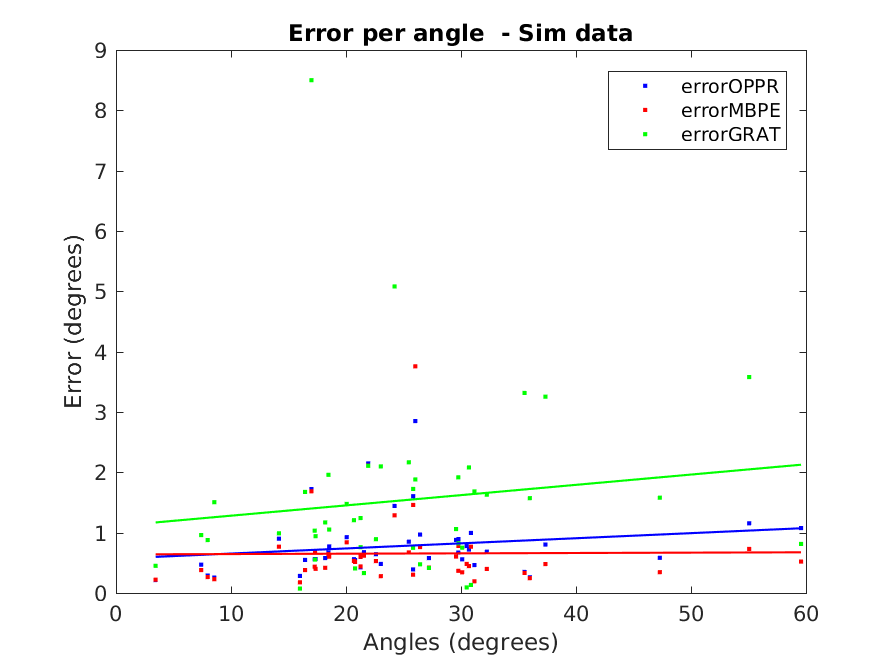
\includegraphics[width=\textwidth]{images/sim/45angle.png}
	\captionof{figure}{Error per saccade amplitude (in degrees) under simulation.}
	\label{cha5:sec1:45angle}
\end{minipage}
\begin{minipage}{0.5\textwidth}
	\centering
	\begin{tabular}{| l | l | l |}
		\hline
		Method & Mean & Standard Deviation \\
		\hline
		OPPR &  0.77 \degree & 0.49 \degree \\
		\hline
		MBPE &  0.65 \degree & 0.60 \degree \\
		\hline
		GRAT &  1.53 \degree & 1.43 \degree \\ 
		\hline
	\end{tabular}
	\captionof{table}{Mean error and standard deviation (in degrees) of the experiment on the left per each method tested}
	\label{cha5:sec1:45anglet}
\end{minipage}\\

\subsubsection{Overview}

Doing the saccades per isolated axis on Experiment 1, demonstrated that there is not a significant difference in the error around a specific coordinate by looking at Table \ref{cha5:sec1:10angleaxist}. Given that, the experiments can comfortably be executed with random saccades around all axis at the same time, which represents the real human eye more accurately.

Table \ref{cha5:sec1:10anglet} and Figure \ref{cha5:sec1:10angle} on Experiment 1, show that for angles under $ 12 \degree $ the mean error is under $0.5 \degree$ for the best two methods, \acrshort{oppr} and \acrshort{mbpe}, whereas for \acrshort{grat} the error is greater. \acrshort{mbpe} seems to be the best method in this case. However, the standard deviation is comparable to the mean for all the methods, alerting instability.

In Table \ref{cha5:sec1:45anglet} and Figure \ref{cha5:sec1:45angle} (Experiment 2), the conditions are all the same except for the amplitude range. Stil \acrshort{mbpe} and \acrshort{oppr} continue to thrive over \acrshort{grat}, this time having \acrshort{oppr} become worse as the saccade amplitude increases. This may be due to the fact that for a bigger saccade, the associated translation creates a larger effect that is not counter acted when using \acrshort{oppr}.

There might be several reasons as to why \acrshort{grat} performs worst than the other algorithms. Because the baseline length is small, the skew translation matrix, that generates the essential matrix together with the rotation, expressed in \ref{sec2:eq:fundm3}, will have values very close to zero, that during intermediate calculus in the minimization can reduce the accuracy of the estimation. Other reason could be that, because the depth, $\lambda$, is not being estimated, opposite to \acrshort{mbpe} (see \ref{fiorenfe}), the leeway to estimate the rotation is reduced, ending up with a poorer guess.
 

\subsection{Variable noise}
\subsubsection{Simulation Parameters}
\begin{itemize}
	\item Maximum Matches : $30$
	\item Good Matches : $50 \%$ of the maximum matches
	\item False Matches : $10 \%$ of maximum matches
	\item Noise $\sigma^2$ : $0-100 \ px$ incrementing $10 \ px$ per iteration
	\item Number of saccades: $45$
	\item Zmin : $0.05 m$
	\item Zmáx : $5 m$
	\item Saccade amplitude $\sigma^2 : 4 \degree $
\end{itemize}
\begin{figure}[ht]
	\centering
	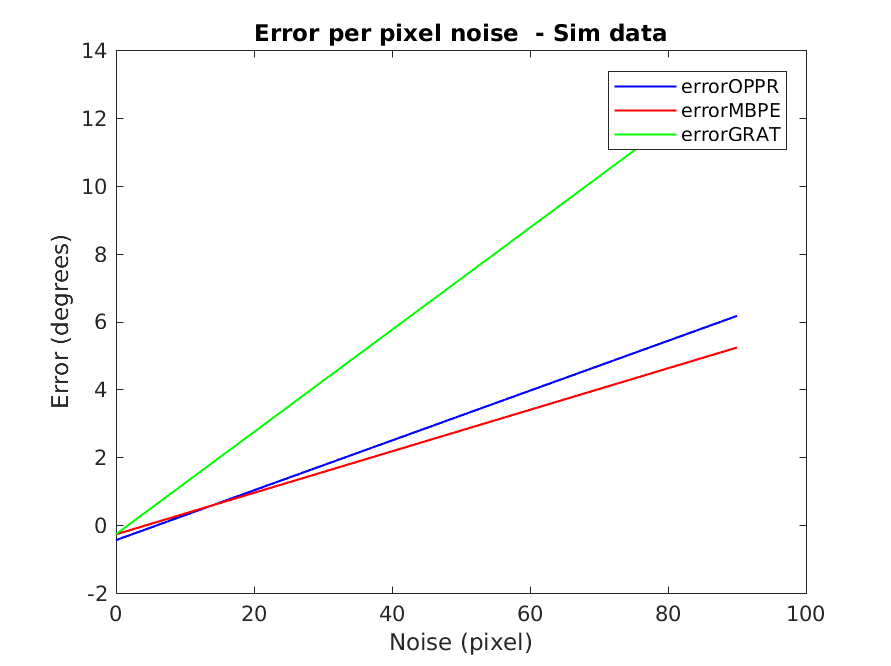
\includegraphics[width=0.5\textwidth]{images/sim/noise.png}
	\captionof{figure}{Error (in degrees) per Gaussian noise in the simulated image (in pixels).}
	\label{cha5:sec1:noise}
\end{figure}
\subsubsection{Overview}

\subsection{Variable baseline}
\subsection{Variable depth}

\subsection{Effect of RANSAC}

\section{Real System}
\subsection{Rotation estimation error}
\subsubsection{Data collection}
\subsubsection{System Parameters}
\begin{itemize}
	\item Maximum Matches : $30$
	\item Good Matches : $50 \%$ of the maximum matches
	\item Zmin : $0.05 m$
	\item Zmáx : $5 m$
	\item Saccade amplitude : random
\end{itemize}
\subsubsection{Experiment 1}
45 saccades were done.\\
\begin{minipage}{0.5\textwidth}
\centering
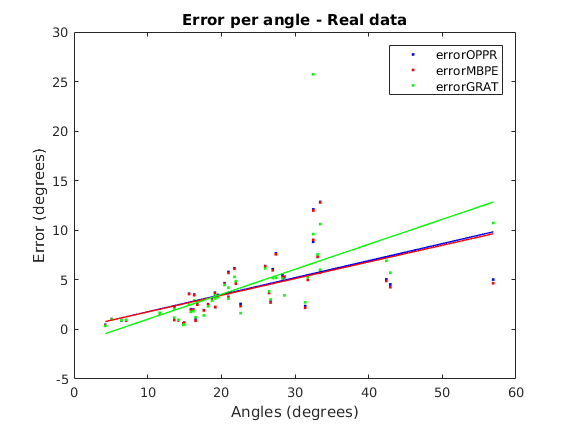
\includegraphics[width=\textwidth]{images/sim/r1angle.png}
\captionof{figure}{Error per saccade amplitude (in degrees) under the real system.}
\label{cha5:sec1:r1angle}
\end{minipage}
\begin{minipage}{0.5\textwidth}
\centering
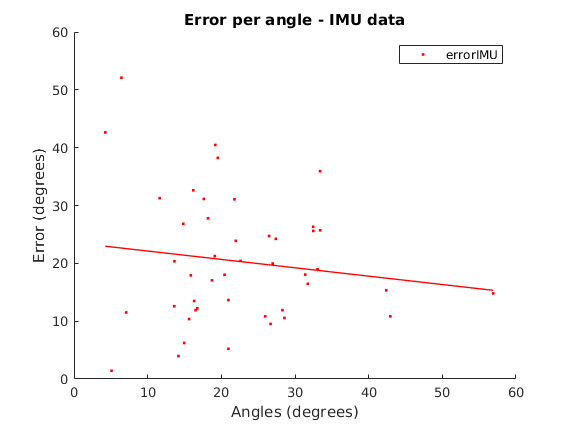
\includegraphics[width=\textwidth]{images/sim/r1angleimu.png}
\captionof{figure}{Error per saccade amplitude (in degrees) under simulation.}
\label{cha5:sec1:r1angleimu}
\end{minipage}\\

\begin{table}
	\centering
\begin{tabular}{| l | l | l |}
	\hline
	Method & Mean & Standard Deviation \\
	\hline
	OPPR &  3.90 \degree & 2.75 \degree \\
	\hline
	MBPE &  3.83 \degree & 2.75 \degree \\
	\hline
	GRAT &  4.13 \degree & 4.09 \degree \\ 
	\hline
	IMU &  20.34 \degree & 10.85 \degree \\ 
	\hline
\end{tabular}
\captionof{table}{Mean error and standard deviation (in degrees) of the experince on the left per each method tested}
\label{cha5:sec1:r1anglet}
\end{table}

Robust estimation detected a $ 94.96 \%$ of bad matches.

\subsubsection{Overview}

\subsubsection{Experiment 2}
32 saccades were done.\\
\begin{minipage}{0.5\textwidth}
	\centering
	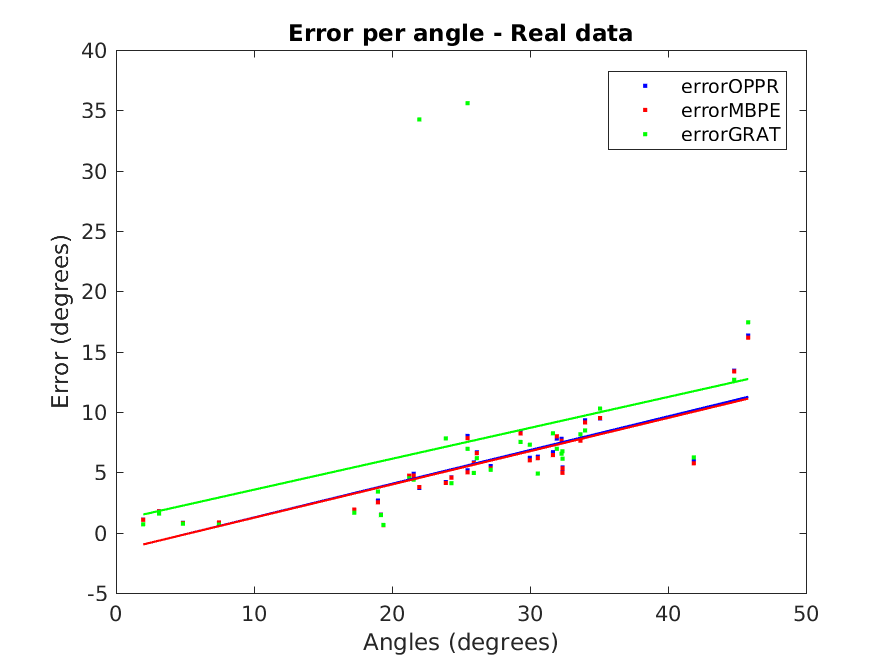
\includegraphics[width=\textwidth]{images/sim/r2angle.png}
	\captionof{figure}{Error per saccade amplitude (in degrees) under simulation.}
	\label{cha5:sec1:r2angle}
\end{minipage}
\begin{minipage}{0.5\textwidth}
	\centering
	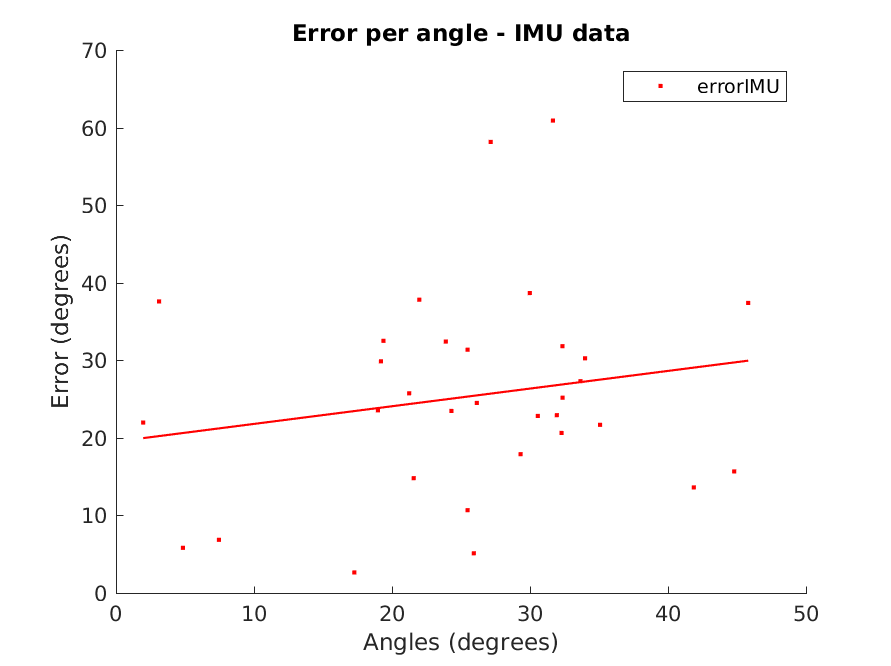
\includegraphics[width=\textwidth]{images/sim/r2angleimu.png}
	\captionof{figure}{Error per saccade amplitude (in degrees) under simulation.}
	\label{cha5:sec1:r2angleimu}
\end{minipage}\\

\begin{table}
	\centering
	\begin{tabular}{| l | l | l |}
		\hline
		Method & Mean & Standard Deviation \\
		\hline
		OPPR &  5.63 \degree & 3.43 \degree \\
		\hline
		MBPE &  5.55 \degree & 3.40 \degree \\
		\hline
		GRAT &  7.57 \degree & 7.79 \degree \\ 
		\hline
		IMU &  25.36 \degree & 13.13 \degree \\ 
		\hline
	\end{tabular}
	\captionof{table}{Mean error and standard deviation (in degrees) of the experince on the left per each method tested}
	\label{cha5:sec1:r2anglet}
\end{table}

Robust estimation detected a $ 93.68 \%$ of bad matches.


\subsubsection{Overview}



\subsection{Effect of RANSAC}

As false matches were generated and Gaussian noise was to the simulation, RANSAC eliminated 


\subsection{Computational speed}